\subsection{UC9 - Visualizzazione dati}
    \label{uc9}
    
    \begin{figure}[htbp]
        \centering
        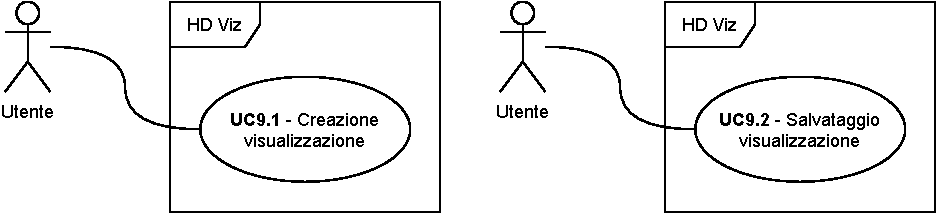
\includegraphics[width=0.9\textwidth]{source/sections/casi-uso/diagrams/uc9.pdf}
        \caption{UC9 - Visualizzazione dati}
        \label{fig:uc9}
    \end{figure}
    
    \begin{itemize}
    \item \textbf{Attore}: utente;
    \item \textbf{Descrizione}: l'utente avvia la visualizzazione del suo dataset secondo le impostazioni;
    \item \textbf{Precondizione}: 
    \begin{itemize}
        \item eseguito l'upload del dataset come matrice $N\times M$ (\hyperref[uc1]{UC1});
        \item selezionato un tipo di visualizzazione (\hyperref[uc2]{UC2});
        \item dati elaborati (\hyperref[uc8]{UC8}).
    \end{itemize}  
    \item \textbf{Postcondizione}: l'applicazione dopo che l'utente dopo ha caricato il suo dataset e selezionato il tipo di visualizzazione, crea la visualizzazione richiesta sul dataset caricato;
    \item \textbf{Scenario Principale}: 
    \begin{enumerate}
        \item l'utente carica il suo dataset (\hyperref[uc1]{UC1});
        \item l'utente seleziona il tipo di visualizzazione tra quelle disponibili (\hyperref[uc2]{UC2});
        \item l'applicazione elabora i dati (\hyperref[uc8]{UC8});
        \item l'applicazione crea la visualizzazione (\hyperref[uc9.1]{UC9.1});
        \item l'utente salva la visualizzazione (\hyperref[uc9.2]{UC9.2}).
    \end{enumerate}
    \end{itemize}
    
    \subsubsection{UC9.1 - Creazione visualizzazione}
    \label{uc9.1}
    \begin{itemize}
    \item \textbf{Attore}: utente;
    \item \textbf{Descrizione}: l'utente avvia la creazione della visualizzazione;
    \item \textbf{Precondizione}: 
    \begin{itemize}
        \item eseguito l'upload del dataset come matrice $N\times M$ (\hyperref[uc1]{UC1});
        \item selezionato un tipo di visualizzazione (\hyperref[uc2]{UC2});
        \item dati elaborati (\hyperref[uc8]{UC8}).
    \end{itemize}  
    \item \textbf{Postcondizione}: l'applicazione dopo che l'utente dopo ha caricato il suo dataset e selezionato il tipo di visualizzazione, crea la visualizzazione a partire dai dati elaborati;
    \item \textbf{Scenario Principale}: 
    \begin{enumerate}
        \item l'utente carica il suo dataset (\hyperref[uc1]{UC1});
        \item l'utente seleziona il tipo di visualizzazione tra quelle disponibili (\hyperref[uc2]{UC2});
        \item l'applicazione elabora i dati (\hyperref[uc8]{UC8});
        \item l'applicazione crea la visualizzazione.
    \end{enumerate}
    \end{itemize}
    
    \subsubsection{UC9.2 - Salvataggio visualizzazione}
    \label{uc9.2}
    \begin{itemize}
    \item \textbf{Attore}: utente;
    \item \textbf{Descrizione}: l'utente salva la visualizzazione;
    \item \textbf{Precondizione}: 
    \begin{itemize}
        \item eseguito l'upload del dataset come matrice $N\times M$ (\hyperref[uc1]{UC1});
        \item selezionato un tipo di visualizzazione (\hyperref[uc2]{UC2});
        \item dati elaborati (\hyperref[uc8]{UC8});
        \item visualizzazione creata (\hyperref[uc9.1]{UC9.1}).
    \end{itemize}  
    \item \textbf{Postcondizione}: l'utente ha salvato la visualizzazione come file immagine PNG;
    \item \textbf{Output}: file PNG con la visualizzazione richiesta;
    \item \textbf{Scenario Principale}: 
    \begin{enumerate}
        \item l'utente carica il suo dataset (\hyperref[uc1]{UC1});
        \item l'utente seleziona il tipo di visualizzazione tra quelle disponibili (\hyperref[uc2]{UC2});
        \item l'applicazione elabora i dati (\hyperref[uc8]{UC8});
        \item l'applicazione crea la visualizzazione;
        \item l'utente salva (cliccando sul pulsante salva) la visualizzazione in formato PNG.
    \end{enumerate}
    \end{itemize}